\documentclass[1p]{elsarticle_modified}
%\bibliographystyle{elsarticle-num}

%\usepackage[colorlinks]{hyperref}
%\usepackage{abbrmath_seonhwa} %\Abb, \Ascr, \Acal ,\Abf, \Afrak
\usepackage{amsfonts}
\usepackage{amssymb}
\usepackage{amsmath}
\usepackage{amsthm}
\usepackage{scalefnt}
\usepackage{amsbsy}
\usepackage{kotex}
\usepackage{caption}
\usepackage{subfig}
\usepackage{color}
\usepackage{graphicx}
\usepackage{xcolor} %% white, black, red, green, blue, cyan, magenta, yellow
\usepackage{float}
\usepackage{setspace}
\usepackage{hyperref}

\usepackage{tikz}
\usetikzlibrary{arrows}

\usepackage{multirow}
\usepackage{array} % fixed length table
\usepackage{hhline}

%%%%%%%%%%%%%%%%%%%%%
\makeatletter
\renewcommand*\env@matrix[1][\arraystretch]{%
	\edef\arraystretch{#1}%
	\hskip -\arraycolsep
	\let\@ifnextchar\new@ifnextchar
	\array{*\c@MaxMatrixCols c}}
\makeatother %https://tex.stackexchange.com/questions/14071/how-can-i-increase-the-line-spacing-in-a-matrix
%%%%%%%%%%%%%%%

\usepackage[normalem]{ulem}

\newcommand{\msout}[1]{\ifmmode\text{\sout{\ensuremath{#1}}}\else\sout{#1}\fi}
%SOURCE: \msout is \stkout macro in https://tex.stackexchange.com/questions/20609/strikeout-in-math-mode

\newcommand{\cancel}[1]{
	\ifmmode
	{\color{red}\msout{#1}}
	\else
	{\color{red}\sout{#1}}
	\fi
}

\newcommand{\add}[1]{
	{\color{blue}\uwave{#1}}
}

\newcommand{\replace}[2]{
	\ifmmode
	{\color{red}\msout{#1}}{\color{blue}\uwave{#2}}
	\else
	{\color{red}\sout{#1}}{\color{blue}\uwave{#2}}
	\fi
}

\newcommand{\Sol}{\mathcal{S}} %segment
\newcommand{\D}{D} %diagram
\newcommand{\A}{\mathcal{A}} %arc


%%%%%%%%%%%%%%%%%%%%%%%%%%%%%5 test

\def\sl{\operatorname{\textup{SL}}(2,\Cbb)}
\def\psl{\operatorname{\textup{PSL}}(2,\Cbb)}
\def\quan{\mkern 1mu \triangleright \mkern 1mu}

\theoremstyle{definition}
\newtheorem{thm}{Theorem}[section]
\newtheorem{prop}[thm]{Proposition}
\newtheorem{lem}[thm]{Lemma}
\newtheorem{ques}[thm]{Question}
\newtheorem{cor}[thm]{Corollary}
\newtheorem{defn}[thm]{Definition}
\newtheorem{exam}[thm]{Example}
\newtheorem{rmk}[thm]{Remark}
\newtheorem{alg}[thm]{Algorithm}

\newcommand{\I}{\sqrt{-1}}
\begin{document}

%\begin{frontmatter}
%
%\title{Boundary parabolic representations of knots up to 8 crossings}
%
%%% Group authors per affiliation:
%\author{Yunhi Cho} 
%\address{Department of Mathematics, University of Seoul, Seoul, Korea}
%\ead{yhcho@uos.ac.kr}
%
%
%\author{Seonhwa Kim} %\fnref{s_kim}}
%\address{Center for Geometry and Physics, Institute for Basic Science, Pohang, 37673, Korea}
%\ead{ryeona17@ibs.re.kr}
%
%\author{Hyuk Kim}
%\address{Department of Mathematical Sciences, Seoul National University, Seoul 08826, Korea}
%\ead{hyukkim@snu.ac.kr}
%
%\author{Seokbeom Yoon}
%\address{Department of Mathematical Sciences, Seoul National University, Seoul, 08826,  Korea}
%\ead{sbyoon15@snu.ac.kr}
%
%\begin{abstract}
%We find all boundary parabolic representation of knots up to 8 crossings.
%
%\end{abstract}
%\begin{keyword}
%    \MSC[2010] 57M25 
%\end{keyword}
%
%\end{frontmatter}

%\linenumbers
%\tableofcontents
%
\newcommand\colored[1]{\textcolor{white}{\rule[-0.35ex]{0.8em}{1.4ex}}\kern-0.8em\color{red} #1}%
%\newcommand\colored[1]{\textcolor{white}{ #1}\kern-2.17ex	\textcolor{white}{ #1}\kern-1.81ex	\textcolor{white}{ #1}\kern-2.15ex\color{red}#1	}

{\Large $\underline{12a_{1229}~(K12a_{1229})}$}

\setlength{\tabcolsep}{10pt}
\renewcommand{\arraystretch}{1.6}
\vspace{1cm}\begin{tabular}{m{100pt}>{\centering\arraybackslash}m{274pt}}
\multirow{5}{120pt}{
	\centering
	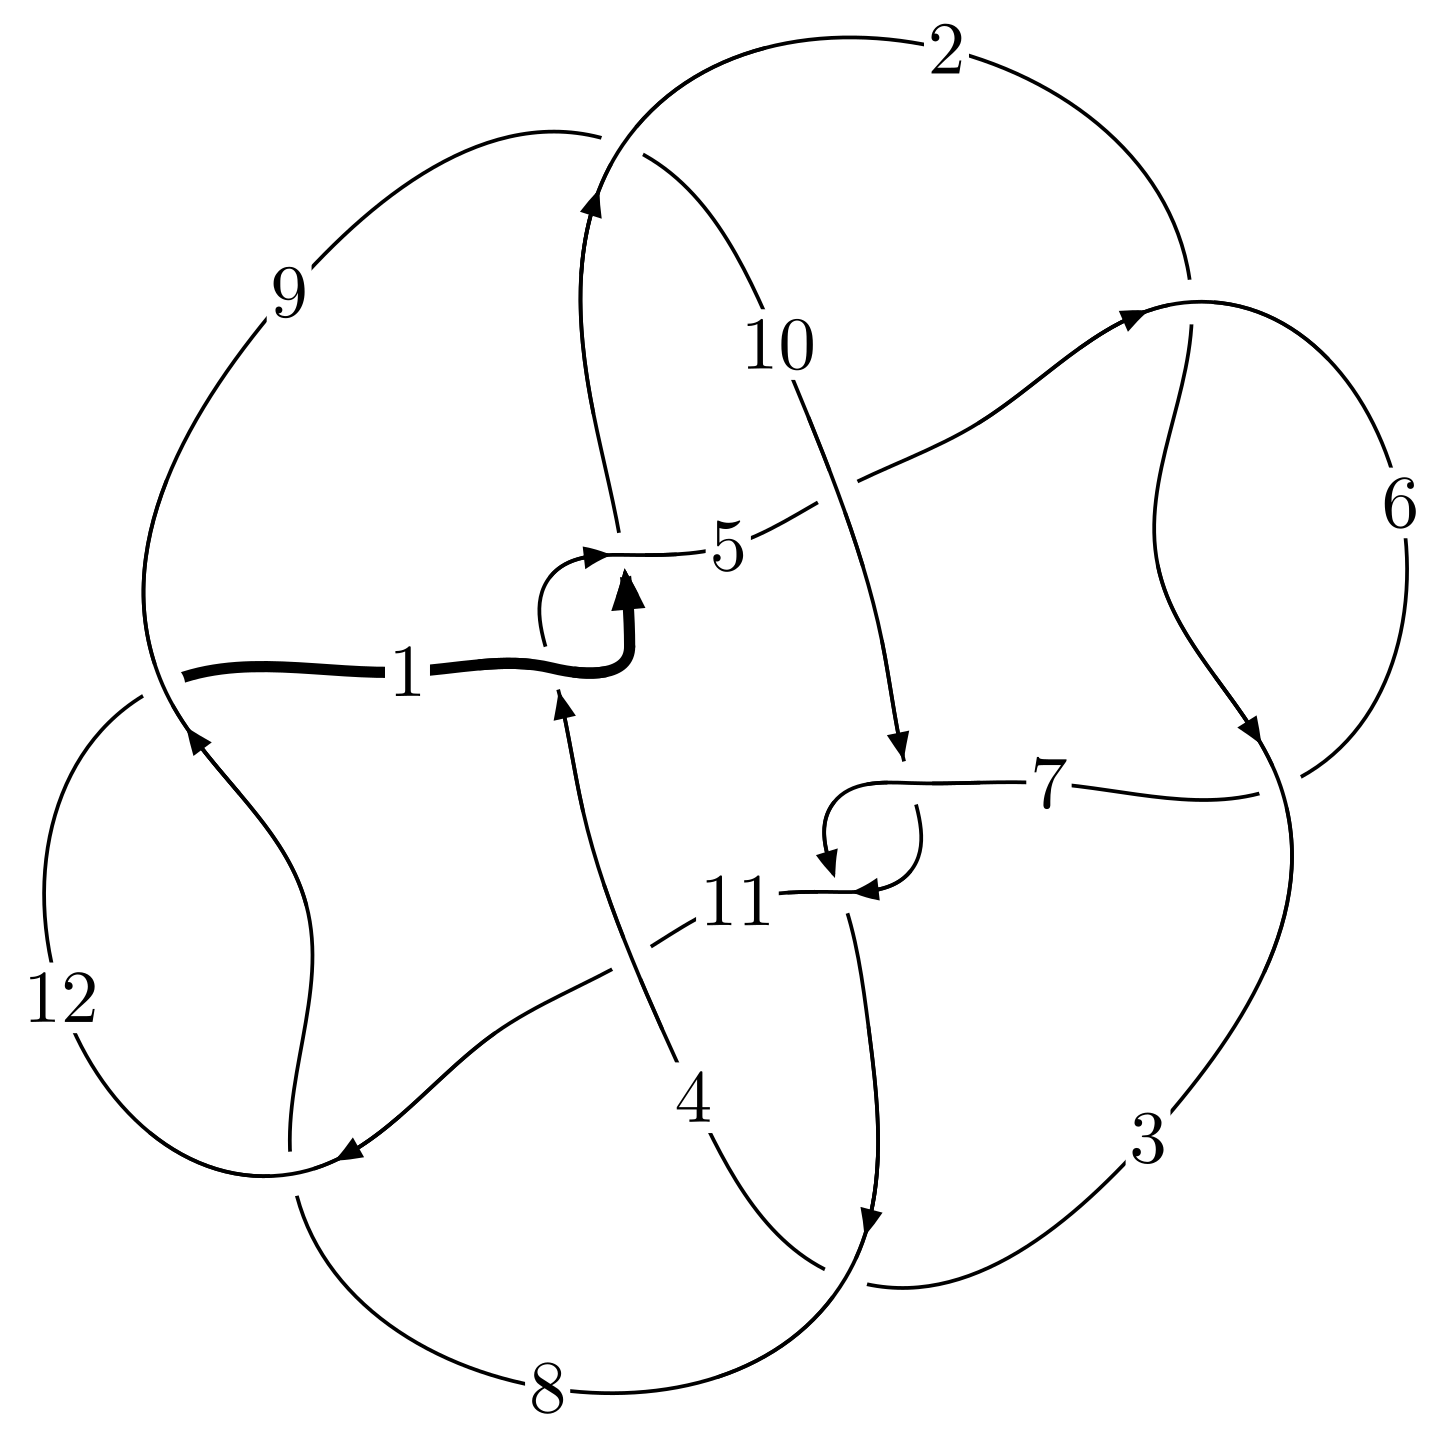
\includegraphics[width=112pt]{../../../GIT/diagram.site/Diagrams/png/2030_12a_1229.png}\\
\ \ \ A knot diagram\footnotemark}&
\allowdisplaybreaks
\textbf{Linearized knot diagam} \\
\cline{2-2}
 &
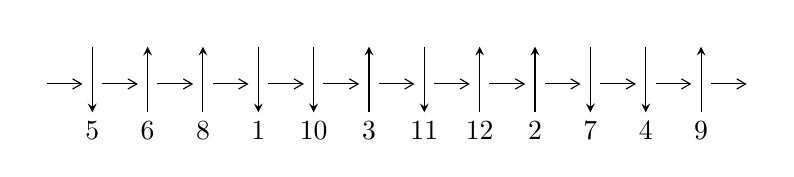
\begin{tikzpicture}[x=20pt, y=17pt]
	% nodes
	\node (C0) at (0, 0) {};
	\node (C1) at (1, 0) {};
	\node (C1U) at (1, +1) {};
	\node (C1D) at (1, -1) {5};

	\node (C2) at (2, 0) {};
	\node (C2U) at (2, +1) {};
	\node (C2D) at (2, -1) {6};

	\node (C3) at (3, 0) {};
	\node (C3U) at (3, +1) {};
	\node (C3D) at (3, -1) {8};

	\node (C4) at (4, 0) {};
	\node (C4U) at (4, +1) {};
	\node (C4D) at (4, -1) {1};

	\node (C5) at (5, 0) {};
	\node (C5U) at (5, +1) {};
	\node (C5D) at (5, -1) {10};

	\node (C6) at (6, 0) {};
	\node (C6U) at (6, +1) {};
	\node (C6D) at (6, -1) {3};

	\node (C7) at (7, 0) {};
	\node (C7U) at (7, +1) {};
	\node (C7D) at (7, -1) {11};

	\node (C8) at (8, 0) {};
	\node (C8U) at (8, +1) {};
	\node (C8D) at (8, -1) {12};

	\node (C9) at (9, 0) {};
	\node (C9U) at (9, +1) {};
	\node (C9D) at (9, -1) {2};

	\node (C10) at (10, 0) {};
	\node (C10U) at (10, +1) {};
	\node (C10D) at (10, -1) {7};

	\node (C11) at (11, 0) {};
	\node (C11U) at (11, +1) {};
	\node (C11D) at (11, -1) {4};

	\node (C12) at (12, 0) {};
	\node (C12U) at (12, +1) {};
	\node (C12D) at (12, -1) {9};
	\node (C13) at (13, 0) {};

	% arrows
	\draw[->,>={angle 60}]
	(C0) edge (C1) (C1) edge (C2) (C2) edge (C3) (C3) edge (C4) (C4) edge (C5) (C5) edge (C6) (C6) edge (C7) (C7) edge (C8) (C8) edge (C9) (C9) edge (C10) (C10) edge (C11) (C11) edge (C12) (C12) edge (C13) ;	\draw[->,>=stealth]
	(C1U) edge (C1D) (C2D) edge (C2U) (C3D) edge (C3U) (C4U) edge (C4D) (C5U) edge (C5D) (C6D) edge (C6U) (C7U) edge (C7D) (C8D) edge (C8U) (C9D) edge (C9U) (C10U) edge (C10D) (C11U) edge (C11D) (C12D) edge (C12U) ;
	\end{tikzpicture} \\
\hhline{~~} \\& 
\textbf{Solving Sequence} \\ \cline{2-2} 
 &
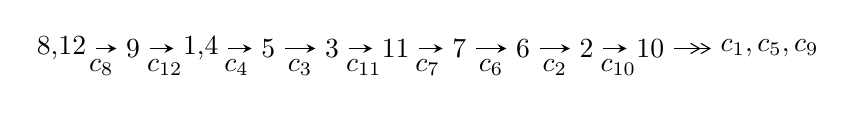
\begin{tikzpicture}[x=23pt, y=7pt]
	% node
	\node (A0) at (-1/8, 0) {8,12};
	\node (A1) at (1, 0) {9};
	\node (A2) at (33/16, 0) {1,4};
	\node (A3) at (25/8, 0) {5};
	\node (A4) at (33/8, 0) {3};
	\node (A5) at (41/8, 0) {11};
	\node (A6) at (49/8, 0) {7};
	\node (A7) at (57/8, 0) {6};
	\node (A8) at (65/8, 0) {2};
	\node (A9) at (73/8, 0) {10};
	\node (C1) at (1/2, -1) {$c_{8}$};
	\node (C2) at (3/2, -1) {$c_{12}$};
	\node (C3) at (21/8, -1) {$c_{4}$};
	\node (C4) at (29/8, -1) {$c_{3}$};
	\node (C5) at (37/8, -1) {$c_{11}$};
	\node (C6) at (45/8, -1) {$c_{7}$};
	\node (C7) at (53/8, -1) {$c_{6}$};
	\node (C8) at (61/8, -1) {$c_{2}$};
	\node (C9) at (69/8, -1) {$c_{10}$};
	\node (A10) at (11, 0) {$c_{1},c_{5},c_{9}$};

	% edge
	\draw[->,>=stealth]	
	(A0) edge (A1) (A1) edge (A2) (A2) edge (A3) (A3) edge (A4) (A4) edge (A5) (A5) edge (A6) (A6) edge (A7) (A7) edge (A8) (A8) edge (A9) ;
	\draw[->>,>={angle 60}]	
	(A9) edge (A10);
\end{tikzpicture} \\ 

\end{tabular} \\

\footnotetext{
The image of knot diagram is generated by the software ``\textbf{Draw programme}" developed by Andrew Bartholomew(\url{http://www.layer8.co.uk/maths/draw/index.htm\#Running-draw}), where we modified some parts for our purpose(\url{https://github.com/CATsTAILs/LinksPainter}).
}\phantom \\ \newline 
\centering \textbf{Ideals for irreducible components\footnotemark of $X_{\text{par}}$} 
 
\begin{align*}
I^u_{1}&=\langle 
-657243 u^{19}+550757 u^{18}+\cdots+15052055 b-22884294,\\
\phantom{I^u_{1}}&\phantom{= \langle  }2745998 u^{19}-1810107 u^{18}+\cdots+885415 a+11576054,\;u^{20}- u^{19}+\cdots+8 u-1\rangle \\
I^u_{2}&=\langle 
1.61625\times10^{510} u^{119}+2.95718\times10^{510} u^{118}+\cdots+2.43355\times10^{509} b+1.95951\times10^{512},\\
\phantom{I^u_{2}}&\phantom{= \langle  }-2.49960\times10^{511} u^{119}-4.27348\times10^{511} u^{118}+\cdots+2.45789\times10^{511} a-1.68445\times10^{513},\\
\phantom{I^u_{2}}&\phantom{= \langle  }u^{120}+u^{119}+\cdots-1207 u-101\rangle \\
I^u_{3}&=\langle 
- u^2+b,\;- u^2+a+1,\;u^6- u^5- u^4+2 u^3- u+1\rangle \\
I^u_{4}&=\langle 
-890375597269 u^{23}+254192032954 u^{22}+\cdots+29055549398 b+3174095591762,\\
\phantom{I^u_{4}}&\phantom{= \langle  }3872069553587 u^{23}-1069682860926 u^{22}+\cdots+29055549398 a-13742313845163,\\
\phantom{I^u_{4}}&\phantom{= \langle  }u^{24}-10 u^{22}+\cdots-11 u-1\rangle \\
\\
\end{align*}
\raggedright * 4 irreducible components of $\dim_{\mathbb{C}}=0$, with total 170 representations.\\
\footnotetext{All coefficients of polynomials are rational numbers. But the coefficients are sometimes approximated in decimal forms when there is not enough margin.}
\newpage
\renewcommand{\arraystretch}{1}
\centering \section*{I. $I^u_{1}= \langle -6.57\times10^{5} u^{19}+5.51\times10^{5} u^{18}+\cdots+1.51\times10^{7} b-2.29\times10^{7},\;2.75\times10^{6} u^{19}-1.81\times10^{6} u^{18}+\cdots+8.85\times10^{5} a+1.16\times10^{7},\;u^{20}- u^{19}+\cdots+8 u-1 \rangle$}
\flushleft \textbf{(i) Arc colorings}\\
\begin{tabular}{m{7pt} m{180pt} m{7pt} m{180pt} }
\flushright $a_{8}=$&$\begin{pmatrix}1\\0\end{pmatrix}$ \\
\flushright $a_{12}=$&$\begin{pmatrix}0\\u\end{pmatrix}$ \\
\flushright $a_{9}=$&$\begin{pmatrix}1\\- u^2\end{pmatrix}$ \\
\flushright $a_{1}=$&$\begin{pmatrix}u\\- u^3+u\end{pmatrix}$ \\
\flushright $a_{4}=$&$\begin{pmatrix}-3.10137 u^{19}+2.04436 u^{18}+\cdots+46.2868 u-13.0742\\0.0436647 u^{19}-0.0365902 u^{18}+\cdots-2.22938 u+1.52034\end{pmatrix}$ \\
\flushright $a_{5}=$&$\begin{pmatrix}-3.38270 u^{19}+1.83814 u^{18}+\cdots+48.5281 u-13.6793\\0.351266 u^{19}+0.114483 u^{18}+\cdots-3.60717 u+1.40274\end{pmatrix}$ \\
\flushright $a_{3}=$&$\begin{pmatrix}-3.14503 u^{19}+2.08095 u^{18}+\cdots+48.5161 u-14.5945\\0.0436647 u^{19}-0.0365902 u^{18}+\cdots-2.22938 u+1.52034\end{pmatrix}$ \\
\flushright $a_{11}=$&$\begin{pmatrix}4.34974 u^{19}-3.12294 u^{18}+\cdots-60.9551 u+17.5138\\-0.605158 u^{19}+0.323827 u^{18}+\cdots+7.26222 u-2.59996\end{pmatrix}$ \\
\flushright $a_{7}=$&$\begin{pmatrix}5.75707 u^{19}-4.24667 u^{18}+\cdots-87.5291 u+27.3276\\-0.400467 u^{19}+0.658924 u^{18}+\cdots+11.8243 u-4.07902\end{pmatrix}$ \\
\flushright $a_{6}=$&$\begin{pmatrix}4.69299 u^{19}-3.80267 u^{18}+\cdots-76.9633 u+24.1825\\-0.393392 u^{19}+0.726860 u^{18}+\cdots+12.9953 u-4.03535\end{pmatrix}$ \\
\flushright $a_{2}=$&$\begin{pmatrix}-4.03535 u^{19}+3.64196 u^{18}+\cdots+61.8775 u-19.2875\\-0.289803 u^{19}-0.784497 u^{18}+\cdots-1.34116 u+1.91374\end{pmatrix}$ \\
\flushright $a_{10}=$&$\begin{pmatrix}-5.17324 u^{19}+4.24751 u^{18}+\cdots+75.3851 u-25.4465\\1.22379 u^{19}-0.813102 u^{18}+\cdots-14.2496 u+4.29959\end{pmatrix}$\\&\end{tabular}
\flushleft \textbf{(ii) Obstruction class $= -1$}\\~\\
\flushleft \textbf{(iii) Cusp Shapes $= -\frac{25801680}{3010411} u^{19}+\frac{13740304}{3010411} u^{18}+\cdots+\frac{265194524}{3010411} u-\frac{69023780}{3010411}$}\\~\\
\newpage\renewcommand{\arraystretch}{1}
\flushleft \textbf{(iv) u-Polynomials at the component}\newline \\
\begin{tabular}{m{50pt}|m{274pt}}
Crossings & \hspace{64pt}u-Polynomials at each crossing \\
\hline $$\begin{aligned}c_{1},c_{4},c_{7}\\c_{10}\end{aligned}$$&$\begin{aligned}
&u^{20}+u^{19}+\cdots-8 u-1
\end{aligned}$\\
\hline $$\begin{aligned}c_{2},c_{6},c_{8}\\c_{12}\end{aligned}$$&$\begin{aligned}
&u^{20}- u^{19}+\cdots+8 u-1
\end{aligned}$\\
\hline $$\begin{aligned}c_{3},c_{9}\end{aligned}$$&$\begin{aligned}
&u^{20}+3 u^{19}+\cdots-4 u+1
\end{aligned}$\\
\hline $$\begin{aligned}c_{5},c_{11}\end{aligned}$$&$\begin{aligned}
&u^{20}-3 u^{19}+\cdots+4 u+1
\end{aligned}$\\
\hline
\end{tabular}\\~\\
\newpage\renewcommand{\arraystretch}{1}
\flushleft \textbf{(v) Riley Polynomials at the component}\newline \\
\begin{tabular}{m{50pt}|m{274pt}}
Crossings & \hspace{64pt}Riley Polynomials at each crossing \\
\hline $$\begin{aligned}c_{1},c_{2},c_{4}\\c_{6},c_{7},c_{8}\\c_{10},c_{12}\end{aligned}$$&$\begin{aligned}
&y^{20}-21 y^{19}+\cdots-22 y+1
\end{aligned}$\\
\hline $$\begin{aligned}c_{3},c_{5},c_{9}\\c_{11}\end{aligned}$$&$\begin{aligned}
&y^{20}-9 y^{19}+\cdots-58 y+1
\end{aligned}$\\
\hline
\end{tabular}\\~\\
\newpage\flushleft \textbf{(vi) Complex Volumes and Cusp Shapes}
$$\begin{array}{c|c|c}  
\text{Solutions to }I^u_{1}& \I (\text{vol} + \sqrt{-1}CS) & \text{Cusp shape}\\
 \hline 
\begin{aligned}
u &= -0.937024 + 0.450242 I \\
a &= -0.384605 - 0.337640 I \\
b &= -0.751635 - 1.117870 I\end{aligned}
 & -3.67791 - 3.10330 I & -3.51583 + 4.92617 I \\ \hline\begin{aligned}
u &= -0.937024 - 0.450242 I \\
a &= -0.384605 + 0.337640 I \\
b &= -0.751635 + 1.117870 I\end{aligned}
 & -3.67791 + 3.10330 I & -3.51583 - 4.92617 I \\ \hline\begin{aligned}
u &= -0.942219\phantom{ +0.000000I} \\
a &= -1.69416\phantom{ +0.000000I} \\
b &= \phantom{-}1.71447\phantom{ +0.000000I}\end{aligned}
 & -6.37866\phantom{ +0.000000I} & \phantom{-}3.70440\phantom{ +0.000000I} \\ \hline\begin{aligned}
u &= -0.090437 + 1.100790 I \\
a &= \phantom{-}0.357560 - 1.069910 I \\
b &= \phantom{-}0.819196 - 1.038580 I\end{aligned}
 & -9.29934 - 6.91821 I & -7.59605 + 5.76583 I \\ \hline\begin{aligned}
u &= -0.090437 - 1.100790 I \\
a &= \phantom{-}0.357560 + 1.069910 I \\
b &= \phantom{-}0.819196 + 1.038580 I\end{aligned}
 & -9.29934 + 6.91821 I & -7.59605 - 5.76583 I \\ \hline\begin{aligned}
u &= \phantom{-}1.162070 + 0.230203 I \\
a &= \phantom{-}0.805749 + 0.802349 I \\
b &= -0.512403 - 0.143211 I\end{aligned}
 & \phantom{-}3.67791 + 3.10330 I & \phantom{-}3.51583 - 4.92617 I \\ \hline\begin{aligned}
u &= \phantom{-}1.162070 - 0.230203 I \\
a &= \phantom{-}0.805749 - 0.802349 I \\
b &= -0.512403 + 0.143211 I\end{aligned}
 & \phantom{-}3.67791 - 3.10330 I & \phantom{-}3.51583 + 4.92617 I \\ \hline\begin{aligned}
u &= \phantom{-}0.692420 + 0.175493 I \\
a &= -0.62416 - 1.52463 I \\
b &= \phantom{-}0.164619 - 1.165220 I\end{aligned}
 & \phantom{-0.000000 -}0.945117 I & \phantom{-0.000000 } 0. - 6.62663 I \\ \hline\begin{aligned}
u &= \phantom{-}0.692420 - 0.175493 I \\
a &= -0.62416 + 1.52463 I \\
b &= \phantom{-}0.164619 + 1.165220 I\end{aligned}
 & \phantom{-0.000000 } -0.945117 I & \phantom{-0.000000 -}0. + 6.62663 I \\ \hline\begin{aligned}
u &= -1.357150 + 0.312893 I \\
a &= \phantom{-}0.405622 + 0.858786 I \\
b &= -1.145400 + 0.490357 I\end{aligned}
 & \phantom{-}9.29934 - 6.91821 I & \phantom{-}7.59605 + 5.76583 I\\
 \hline 
 \end{array}$$\newpage$$\begin{array}{c|c|c}  
\text{Solutions to }I^u_{1}& \I (\text{vol} + \sqrt{-1}CS) & \text{Cusp shape}\\
 \hline 
\begin{aligned}
u &= -1.357150 - 0.312893 I \\
a &= \phantom{-}0.405622 - 0.858786 I \\
b &= -1.145400 - 0.490357 I\end{aligned}
 & \phantom{-}9.29934 + 6.91821 I & \phantom{-}7.59605 - 5.76583 I \\ \hline\begin{aligned}
u &= \phantom{-}1.43028 + 0.61765 I \\
a &= \phantom{-}0.527948 - 0.948587 I \\
b &= -1.34101 - 1.03066 I\end{aligned}
 & \phantom{-0.000000 -}19.4225 I & \phantom{-0.000000 } 0. - 9.88055 I \\ \hline\begin{aligned}
u &= \phantom{-}1.43028 - 0.61765 I \\
a &= \phantom{-}0.527948 + 0.948587 I \\
b &= -1.34101 + 1.03066 I\end{aligned}
 & \phantom{-0.000000 } -19.4225 I & \phantom{-0.000000 -}0. + 9.88055 I \\ \hline\begin{aligned}
u &= \phantom{-}1.56596\phantom{ +0.000000I} \\
a &= -0.0875994\phantom{ +0.000000I} \\
b &= -0.956582\phantom{ +0.000000I}\end{aligned}
 & \phantom{-}1.07560\phantom{ +0.000000I} & \phantom{-}8.20320\phantom{ +0.000000I} \\ \hline\begin{aligned}
u &= \phantom{-}1.57822\phantom{ +0.000000I} \\
a &= -0.828201\phantom{ +0.000000I} \\
b &= \phantom{-}1.36600\phantom{ +0.000000I}\end{aligned}
 & \phantom{-}8.74433\phantom{ +0.000000I} & \phantom{-}11.3570\phantom{ +0.000000I} \\ \hline\begin{aligned}
u &= \phantom{-}0.141085 + 0.364901 I \\
a &= \phantom{-}0.816431 + 1.084900 I \\
b &= \phantom{-}0.280693 + 0.450979 I\end{aligned}
 & \phantom{-0.000000 -}0.971689 I & \phantom{-0.000000 } 0. - 6.75018 I \\ \hline\begin{aligned}
u &= \phantom{-}0.141085 - 0.364901 I \\
a &= \phantom{-}0.816431 - 1.084900 I \\
b &= \phantom{-}0.280693 - 0.450979 I\end{aligned}
 & \phantom{-0.000000 } -0.971689 I & \phantom{-0.000000 -}0. + 6.75018 I \\ \hline\begin{aligned}
u &= -1.69718\phantom{ +0.000000I} \\
a &= -0.563631\phantom{ +0.000000I} \\
b &= \phantom{-}0.137177\phantom{ +0.000000I}\end{aligned}
 & -1.07560\phantom{ +0.000000I} & -8.20320\phantom{ +0.000000I} \\ \hline\begin{aligned}
u &= \phantom{-}0.207256\phantom{ +0.000000I} \\
a &= -6.59087\phantom{ +0.000000I} \\
b &= \phantom{-}1.30709\phantom{ +0.000000I}\end{aligned}
 & -8.74433\phantom{ +0.000000I} & -11.3570\phantom{ +0.000000I} \\ \hline\begin{aligned}
u &= -1.79455\phantom{ +0.000000I} \\
a &= \phantom{-}0.955379\phantom{ +0.000000I} \\
b &= -1.59627\phantom{ +0.000000I}\end{aligned}
 & \phantom{-}6.37866\phantom{ +0.000000I} & -3.70440\phantom{ +0.000000I}\\
 \hline 
 \end{array}$$\newpage\newpage\renewcommand{\arraystretch}{1}
\centering \section*{II. $I^u_{2}= \langle 1.62\times10^{510} u^{119}+2.96\times10^{510} u^{118}+\cdots+2.43\times10^{509} b+1.96\times10^{512},\;-2.50\times10^{511} u^{119}-4.27\times10^{511} u^{118}+\cdots+2.46\times10^{511} a-1.68\times10^{513},\;u^{120}+u^{119}+\cdots-1207 u-101 \rangle$}
\flushleft \textbf{(i) Arc colorings}\\
\begin{tabular}{m{7pt} m{180pt} m{7pt} m{180pt} }
\flushright $a_{8}=$&$\begin{pmatrix}1\\0\end{pmatrix}$ \\
\flushright $a_{12}=$&$\begin{pmatrix}0\\u\end{pmatrix}$ \\
\flushright $a_{9}=$&$\begin{pmatrix}1\\- u^2\end{pmatrix}$ \\
\flushright $a_{1}=$&$\begin{pmatrix}u\\- u^3+u\end{pmatrix}$ \\
\flushright $a_{4}=$&$\begin{pmatrix}1.01697 u^{119}+1.73868 u^{118}+\cdots+1250.63 u+68.5325\\-6.64154 u^{119}-12.1517 u^{118}+\cdots-10621.1 u-805.207\end{pmatrix}$ \\
\flushright $a_{5}=$&$\begin{pmatrix}5.75809 u^{119}+10.3986 u^{118}+\cdots+8895.14 u+648.617\\-5.12212 u^{119}-9.38884 u^{118}+\cdots-8185.42 u-620.921\end{pmatrix}$ \\
\flushright $a_{3}=$&$\begin{pmatrix}7.65852 u^{119}+13.8904 u^{118}+\cdots+11871.7 u+873.739\\-6.64154 u^{119}-12.1517 u^{118}+\cdots-10621.1 u-805.207\end{pmatrix}$ \\
\flushright $a_{11}=$&$\begin{pmatrix}-1.11875 u^{119}-2.64304 u^{118}+\cdots-1268.92 u-121.688\\-2.20452 u^{119}-4.10235 u^{118}+\cdots-3190.02 u-238.655\end{pmatrix}$ \\
\flushright $a_{7}=$&$\begin{pmatrix}-3.36432 u^{119}-6.52962 u^{118}+\cdots-4543.21 u-344.737\\3.27162 u^{119}+6.24353 u^{118}+\cdots+4661.08 u+355.334\end{pmatrix}$ \\
\flushright $a_{6}=$&$\begin{pmatrix}10.5896 u^{119}+19.1853 u^{118}+\cdots+16483.5 u+1214.74\\-8.57234 u^{119}-15.5835 u^{118}+\cdots-13957.2 u-1056.32\end{pmatrix}$ \\
\flushright $a_{2}=$&$\begin{pmatrix}-11.1962 u^{119}-20.8532 u^{118}+\cdots-16571.6 u-1239.72\\8.28041 u^{119}+15.5128 u^{118}+\cdots+12526.9 u+951.367\end{pmatrix}$ \\
\flushright $a_{10}=$&$\begin{pmatrix}-2.27197 u^{119}-4.78743 u^{118}+\cdots-2978.31 u-251.605\\1.58455 u^{119}+2.95319 u^{118}+\cdots+2593.22 u+203.741\end{pmatrix}$\\&\end{tabular}
\flushleft \textbf{(ii) Obstruction class $= -1$}\\~\\
\flushleft \textbf{(iii) Cusp Shapes $= -36.0800 u^{119}-67.2942 u^{118}+\cdots-54086.0 u-4089.21$}\\~\\
\newpage\renewcommand{\arraystretch}{1}
\flushleft \textbf{(iv) u-Polynomials at the component}\newline \\
\begin{tabular}{m{50pt}|m{274pt}}
Crossings & \hspace{64pt}u-Polynomials at each crossing \\
\hline $$\begin{aligned}c_{1},c_{4},c_{7}\\c_{10}\end{aligned}$$&$\begin{aligned}
&u^{120}- u^{119}+\cdots+1207 u-101
\end{aligned}$\\
\hline $$\begin{aligned}c_{2},c_{6},c_{8}\\c_{12}\end{aligned}$$&$\begin{aligned}
&u^{120}+u^{119}+\cdots-1207 u-101
\end{aligned}$\\
\hline $$\begin{aligned}c_{3},c_{9}\end{aligned}$$&$\begin{aligned}
&u^{120}-7 u^{117}+\cdots-175 u-575
\end{aligned}$\\
\hline $$\begin{aligned}c_{5},c_{11}\end{aligned}$$&$\begin{aligned}
&u^{120}+7 u^{117}+\cdots+175 u-575
\end{aligned}$\\
\hline
\end{tabular}\\~\\
\newpage\renewcommand{\arraystretch}{1}
\flushleft \textbf{(v) Riley Polynomials at the component}\newline \\
\begin{tabular}{m{50pt}|m{274pt}}
Crossings & \hspace{64pt}Riley Polynomials at each crossing \\
\hline $$\begin{aligned}c_{1},c_{2},c_{4}\\c_{6},c_{7},c_{8}\\c_{10},c_{12}\end{aligned}$$&$\begin{aligned}
&y^{120}-73 y^{119}+\cdots-569059 y+10201
\end{aligned}$\\
\hline $$\begin{aligned}c_{3},c_{5},c_{9}\\c_{11}\end{aligned}$$&$\begin{aligned}
&y^{120}+86 y^{118}+\cdots-5688625 y+330625
\end{aligned}$\\
\hline
\end{tabular}\\~\\
\newpage\flushleft \textbf{(vi) Complex Volumes and Cusp Shapes}
$$\begin{array}{c|c|c}  
\text{Solutions to }I^u_{2}& \I (\text{vol} + \sqrt{-1}CS) & \text{Cusp shape}\\
 \hline 
\begin{aligned}
u &= \phantom{-}0.571383 + 0.817824 I \\
a &= -0.337837 - 0.625440 I \\
b &= -0.767765 - 0.308435 I\end{aligned}
 & \phantom{-}3.58665 + 3.20085 I & \phantom{-0.000000 } 0 \\ \hline\begin{aligned}
u &= \phantom{-}0.571383 - 0.817824 I \\
a &= -0.337837 + 0.625440 I \\
b &= -0.767765 + 0.308435 I\end{aligned}
 & \phantom{-}3.58665 - 3.20085 I & \phantom{-0.000000 } 0 \\ \hline\begin{aligned}
u &= \phantom{-}1.015410 + 0.099318 I \\
a &= \phantom{-}0.775962 - 0.840114 I \\
b &= -1.62880 - 1.21221 I\end{aligned}
 & \phantom{-}0.87063 + 4.37653 I & \phantom{-0.000000 } 0 \\ \hline\begin{aligned}
u &= \phantom{-}1.015410 - 0.099318 I \\
a &= \phantom{-}0.775962 + 0.840114 I \\
b &= -1.62880 + 1.21221 I\end{aligned}
 & \phantom{-}0.87063 - 4.37653 I & \phantom{-0.000000 } 0 \\ \hline\begin{aligned}
u &= \phantom{-}1.029960 + 0.108703 I \\
a &= \phantom{-}1.44044 + 1.01116 I \\
b &= -1.120920 + 0.163726 I\end{aligned}
 & \phantom{-}3.43093 + 4.34668 I & \phantom{-0.000000 } 0 \\ \hline\begin{aligned}
u &= \phantom{-}1.029960 - 0.108703 I \\
a &= \phantom{-}1.44044 - 1.01116 I \\
b &= -1.120920 - 0.163726 I\end{aligned}
 & \phantom{-}3.43093 - 4.34668 I & \phantom{-0.000000 } 0 \\ \hline\begin{aligned}
u &= -0.376706 + 0.970628 I \\
a &= \phantom{-}0.709879 + 0.393674 I \\
b &= \phantom{-}0.541187 + 0.911081 I\end{aligned}
 & -0.31640 + 3.81201 I & \phantom{-0.000000 } 0 \\ \hline\begin{aligned}
u &= -0.376706 - 0.970628 I \\
a &= \phantom{-}0.709879 - 0.393674 I \\
b &= \phantom{-}0.541187 - 0.911081 I\end{aligned}
 & -0.31640 - 3.81201 I & \phantom{-0.000000 } 0 \\ \hline\begin{aligned}
u &= \phantom{-}0.929577 + 0.130081 I \\
a &= -0.52107 - 1.59976 I \\
b &= \phantom{-}0.495079 - 0.392935 I\end{aligned}
 & \phantom{-0.000000 -}0.419089 I & \phantom{-0.000000 } 0 \\ \hline\begin{aligned}
u &= \phantom{-}0.929577 - 0.130081 I \\
a &= -0.52107 + 1.59976 I \\
b &= \phantom{-}0.495079 + 0.392935 I\end{aligned}
 & \phantom{-0.000000 } -0.419089 I & \phantom{-0.000000 } 0\\
 \hline 
 \end{array}$$\newpage$$\begin{array}{c|c|c}  
\text{Solutions to }I^u_{2}& \I (\text{vol} + \sqrt{-1}CS) & \text{Cusp shape}\\
 \hline 
\begin{aligned}
u &= \phantom{-}1.024900 + 0.276881 I \\
a &= \phantom{-}0.15555 - 1.79236 I \\
b &= -0.206866 - 0.464700 I\end{aligned}
 & \phantom{-}0.159819 + 0.791393 I & \phantom{-0.000000 } 0 \\ \hline\begin{aligned}
u &= \phantom{-}1.024900 - 0.276881 I \\
a &= \phantom{-}0.15555 + 1.79236 I \\
b &= -0.206866 + 0.464700 I\end{aligned}
 & \phantom{-}0.159819 - 0.791393 I & \phantom{-0.000000 } 0 \\ \hline\begin{aligned}
u &= \phantom{-}0.917589 + 0.114336 I \\
a &= -1.05262 - 1.82444 I \\
b &= \phantom{-}0.499926 - 0.525485 I\end{aligned}
 & -0.159819 + 0.791393 I & \phantom{-0.000000 } 0 \\ \hline\begin{aligned}
u &= \phantom{-}0.917589 - 0.114336 I \\
a &= -1.05262 + 1.82444 I \\
b &= \phantom{-}0.499926 + 0.525485 I\end{aligned}
 & -0.159819 - 0.791393 I & \phantom{-0.000000 } 0 \\ \hline\begin{aligned}
u &= -0.220382 + 1.055820 I \\
a &= -0.691368 - 0.822797 I \\
b &= -0.802424 - 0.803524 I\end{aligned}
 & -5.81721 + 4.62194 I & \phantom{-0.000000 } 0 \\ \hline\begin{aligned}
u &= -0.220382 - 1.055820 I \\
a &= -0.691368 + 0.822797 I \\
b &= -0.802424 + 0.803524 I\end{aligned}
 & -5.81721 - 4.62194 I & \phantom{-0.000000 } 0 \\ \hline\begin{aligned}
u &= -0.430102 + 0.999454 I \\
a &= -0.703162 - 0.687615 I \\
b &= \phantom{-}0.067673 - 1.048070 I\end{aligned}
 & -2.63314 + 3.37265 I & \phantom{-0.000000 } 0 \\ \hline\begin{aligned}
u &= -0.430102 - 0.999454 I \\
a &= -0.703162 + 0.687615 I \\
b &= \phantom{-}0.067673 + 1.048070 I\end{aligned}
 & -2.63314 - 3.37265 I & \phantom{-0.000000 } 0 \\ \hline\begin{aligned}
u &= -0.890569 + 0.149096 I \\
a &= \phantom{-}1.29257 + 1.47928 I \\
b &= -0.971229 + 0.609138 I\end{aligned}
 & -2.63314 - 3.37265 I & \phantom{-0.000000 } 0 \\ \hline\begin{aligned}
u &= -0.890569 - 0.149096 I \\
a &= \phantom{-}1.29257 - 1.47928 I \\
b &= -0.971229 - 0.609138 I\end{aligned}
 & -2.63314 + 3.37265 I & \phantom{-0.000000 } 0\\
 \hline 
 \end{array}$$\newpage$$\begin{array}{c|c|c}  
\text{Solutions to }I^u_{2}& \I (\text{vol} + \sqrt{-1}CS) & \text{Cusp shape}\\
 \hline 
\begin{aligned}
u &= -1.085370 + 0.245075 I \\
a &= \phantom{-}0.070673 - 0.888919 I \\
b &= -0.472794 - 0.687874 I\end{aligned}
 & -0.31640 - 3.81201 I & \phantom{-0.000000 } 0 \\ \hline\begin{aligned}
u &= -1.085370 - 0.245075 I \\
a &= \phantom{-}0.070673 + 0.888919 I \\
b &= -0.472794 + 0.687874 I\end{aligned}
 & -0.31640 + 3.81201 I & \phantom{-0.000000 } 0 \\ \hline\begin{aligned}
u &= -1.121070 + 0.002297 I \\
a &= -0.676952 + 0.628951 I \\
b &= \phantom{-}1.348580 + 0.398307 I\end{aligned}
 & \phantom{-}5.58448 + 0.82681 I & \phantom{-0.000000 } 0 \\ \hline\begin{aligned}
u &= -1.121070 - 0.002297 I \\
a &= -0.676952 - 0.628951 I \\
b &= \phantom{-}1.348580 - 0.398307 I\end{aligned}
 & \phantom{-}5.58448 - 0.82681 I & \phantom{-0.000000 } 0 \\ \hline\begin{aligned}
u &= \phantom{-}0.956984 + 0.655205 I \\
a &= -0.348777 + 0.259561 I \\
b &= -0.45047 + 1.69807 I\end{aligned}
 & -2.49209 + 10.34980 I & \phantom{-0.000000 } 0 \\ \hline\begin{aligned}
u &= \phantom{-}0.956984 - 0.655205 I \\
a &= -0.348777 - 0.259561 I \\
b &= -0.45047 - 1.69807 I\end{aligned}
 & -2.49209 - 10.34980 I & \phantom{-0.000000 } 0 \\ \hline\begin{aligned}
u &= \phantom{-}0.838810 + 0.018028 I \\
a &= -0.022628 - 0.308718 I \\
b &= -0.73721 + 1.56066 I\end{aligned}
 & \phantom{-}0.20224 - 3.55721 I & \phantom{-0.000000 } 0 \\ \hline\begin{aligned}
u &= \phantom{-}0.838810 - 0.018028 I \\
a &= -0.022628 + 0.308718 I \\
b &= -0.73721 - 1.56066 I\end{aligned}
 & \phantom{-}0.20224 + 3.55721 I & \phantom{-0.000000 } 0 \\ \hline\begin{aligned}
u &= \phantom{-}1.056600 + 0.487993 I \\
a &= \phantom{-}0.272721 - 0.127124 I \\
b &= \phantom{-}0.81363 - 1.35709 I\end{aligned}
 & -5.81721 + 4.62194 I & \phantom{-0.000000 } 0 \\ \hline\begin{aligned}
u &= \phantom{-}1.056600 - 0.487993 I \\
a &= \phantom{-}0.272721 + 0.127124 I \\
b &= \phantom{-}0.81363 + 1.35709 I\end{aligned}
 & -5.81721 - 4.62194 I & \phantom{-0.000000 } 0\\
 \hline 
 \end{array}$$\newpage$$\begin{array}{c|c|c}  
\text{Solutions to }I^u_{2}& \I (\text{vol} + \sqrt{-1}CS) & \text{Cusp shape}\\
 \hline 
\begin{aligned}
u &= -1.150200 + 0.209306 I \\
a &= -0.63913 + 1.36002 I \\
b &= \phantom{-}0.503840 - 0.019875 I\end{aligned}
 & \phantom{-}2.49209 - 10.34980 I & \phantom{-0.000000 } 0 \\ \hline\begin{aligned}
u &= -1.150200 - 0.209306 I \\
a &= -0.63913 - 1.36002 I \\
b &= \phantom{-}0.503840 + 0.019875 I\end{aligned}
 & \phantom{-}2.49209 + 10.34980 I & \phantom{-0.000000 } 0 \\ \hline\begin{aligned}
u &= -1.163030 + 0.207546 I \\
a &= -0.338959 - 0.777400 I \\
b &= \phantom{-}0.769100 - 0.908473 I\end{aligned}
 & \phantom{-}3.58665 - 3.20085 I & \phantom{-0.000000 } 0 \\ \hline\begin{aligned}
u &= -1.163030 - 0.207546 I \\
a &= -0.338959 + 0.777400 I \\
b &= \phantom{-}0.769100 + 0.908473 I\end{aligned}
 & \phantom{-}3.58665 + 3.20085 I & \phantom{-0.000000 } 0 \\ \hline\begin{aligned}
u &= -1.18600\phantom{ +0.000000I} \\
a &= \phantom{-}0.491723\phantom{ +0.000000I} \\
b &= \phantom{-}0.878739\phantom{ +0.000000I}\end{aligned}
 & -5.62510\phantom{ +0.000000I} & \phantom{-0.000000 } 0 \\ \hline\begin{aligned}
u &= -1.126730 + 0.405886 I \\
a &= -0.590597 - 0.753377 I \\
b &= \phantom{-}1.37167 - 1.12469 I\end{aligned}
 & \phantom{-}2.63314 - 3.37265 I & \phantom{-0.000000 } 0 \\ \hline\begin{aligned}
u &= -1.126730 - 0.405886 I \\
a &= -0.590597 + 0.753377 I \\
b &= \phantom{-}1.37167 + 1.12469 I\end{aligned}
 & \phantom{-}2.63314 + 3.37265 I & \phantom{-0.000000 } 0 \\ \hline\begin{aligned}
u &= \phantom{-}0.201452 + 0.768382 I \\
a &= -0.00995 + 1.55417 I \\
b &= \phantom{-}1.130110 + 0.779101 I\end{aligned}
 & -8.18473\phantom{ +0.000000I} & \phantom{-0.000000 } 0 \\ \hline\begin{aligned}
u &= \phantom{-}0.201452 - 0.768382 I \\
a &= -0.00995 - 1.55417 I \\
b &= \phantom{-}1.130110 - 0.779101 I\end{aligned}
 & -8.18473\phantom{ +0.000000I} & \phantom{-0.000000 } 0 \\ \hline\begin{aligned}
u &= \phantom{-}0.789728 + 0.065338 I \\
a &= \phantom{-}0.023944 + 1.325150 I \\
b &= -0.989671 + 0.407033 I\end{aligned}
 & \phantom{-}2.63314 - 3.37265 I & \phantom{-0.000000 } 0\\
 \hline 
 \end{array}$$\newpage$$\begin{array}{c|c|c}  
\text{Solutions to }I^u_{2}& \I (\text{vol} + \sqrt{-1}CS) & \text{Cusp shape}\\
 \hline 
\begin{aligned}
u &= \phantom{-}0.789728 - 0.065338 I \\
a &= \phantom{-}0.023944 - 1.325150 I \\
b &= -0.989671 - 0.407033 I\end{aligned}
 & \phantom{-}2.63314 + 3.37265 I & \phantom{-0.000000 } 0 \\ \hline\begin{aligned}
u &= -0.131435 + 1.206100 I \\
a &= -0.321284 - 0.601557 I \\
b &= -0.318465 - 0.633657 I\end{aligned}
 & -3.58665 + 3.20085 I & \phantom{-0.000000 } 0 \\ \hline\begin{aligned}
u &= -0.131435 - 1.206100 I \\
a &= -0.321284 + 0.601557 I \\
b &= -0.318465 + 0.633657 I\end{aligned}
 & -3.58665 - 3.20085 I & \phantom{-0.000000 } 0 \\ \hline\begin{aligned}
u &= \phantom{-}0.705980 + 1.009290 I \\
a &= \phantom{-}0.412700 - 0.821924 I \\
b &= -1.37369 - 1.19804 I\end{aligned}
 & -3.43093 - 4.34668 I & \phantom{-0.000000 } 0 \\ \hline\begin{aligned}
u &= \phantom{-}0.705980 - 1.009290 I \\
a &= \phantom{-}0.412700 + 0.821924 I \\
b &= -1.37369 + 1.19804 I\end{aligned}
 & -3.43093 + 4.34668 I & \phantom{-0.000000 } 0 \\ \hline\begin{aligned}
u &= \phantom{-}1.216130 + 0.235698 I \\
a &= \phantom{-}0.633659 - 1.087890 I \\
b &= -1.02702 - 1.17366 I\end{aligned}
 & \phantom{-0.000000 -}5.66863 I & \phantom{-0.000000 } 0 \\ \hline\begin{aligned}
u &= \phantom{-}1.216130 - 0.235698 I \\
a &= \phantom{-}0.633659 + 1.087890 I \\
b &= -1.02702 + 1.17366 I\end{aligned}
 & \phantom{-0.000000 } -5.66863 I & \phantom{-0.000000 } 0 \\ \hline\begin{aligned}
u &= -0.624516 + 0.424975 I \\
a &= -1.064150 - 0.150384 I \\
b &= -0.569569 - 0.536506 I\end{aligned}
 & -2.93285 + 0.71247 I & \phantom{-0.000000 } 0 \\ \hline\begin{aligned}
u &= -0.624516 - 0.424975 I \\
a &= -1.064150 + 0.150384 I \\
b &= -0.569569 + 0.536506 I\end{aligned}
 & -2.93285 - 0.71247 I & \phantom{-0.000000 } 0 \\ \hline\begin{aligned}
u &= \phantom{-}1.231680 + 0.238226 I \\
a &= \phantom{-}0.364546 - 0.506098 I \\
b &= -0.728486 - 0.358319 I\end{aligned}
 & \phantom{-}2.93285 + 0.71247 I & \phantom{-0.000000 } 0\\
 \hline 
 \end{array}$$\newpage$$\begin{array}{c|c|c}  
\text{Solutions to }I^u_{2}& \I (\text{vol} + \sqrt{-1}CS) & \text{Cusp shape}\\
 \hline 
\begin{aligned}
u &= \phantom{-}1.231680 - 0.238226 I \\
a &= \phantom{-}0.364546 + 0.506098 I \\
b &= -0.728486 + 0.358319 I\end{aligned}
 & \phantom{-}2.93285 - 0.71247 I & \phantom{-0.000000 } 0 \\ \hline\begin{aligned}
u &= -1.253480 + 0.188299 I \\
a &= -0.392247 - 1.303990 I \\
b &= \phantom{-}0.013415 - 0.259364 I\end{aligned}
 & -0.20224 - 3.55721 I & \phantom{-0.000000 } 0 \\ \hline\begin{aligned}
u &= -1.253480 - 0.188299 I \\
a &= -0.392247 + 1.303990 I \\
b &= \phantom{-}0.013415 + 0.259364 I\end{aligned}
 & -0.20224 + 3.55721 I & \phantom{-0.000000 } 0 \\ \hline\begin{aligned}
u &= -1.27931\phantom{ +0.000000I} \\
a &= -0.980199\phantom{ +0.000000I} \\
b &= \phantom{-}1.55109\phantom{ +0.000000I}\end{aligned}
 & \phantom{-}5.62510\phantom{ +0.000000I} & \phantom{-0.000000 } 0 \\ \hline\begin{aligned}
u &= -1.231390 + 0.385936 I \\
a &= \phantom{-}0.693224 + 0.750299 I \\
b &= -1.72377 + 0.96596 I\end{aligned}
 & \phantom{-}3.43093 - 4.34668 I & \phantom{-0.000000 } 0 \\ \hline\begin{aligned}
u &= -1.231390 - 0.385936 I \\
a &= \phantom{-}0.693224 - 0.750299 I \\
b &= -1.72377 - 0.96596 I\end{aligned}
 & \phantom{-}3.43093 + 4.34668 I & \phantom{-0.000000 } 0 \\ \hline\begin{aligned}
u &= -0.181900 + 0.648976 I \\
a &= -0.02902 + 2.08615 I \\
b &= -0.757463 + 0.706650 I\end{aligned}
 & -5.58448 - 0.82681 I & \phantom{-0.000000 } 0 \\ \hline\begin{aligned}
u &= -0.181900 - 0.648976 I \\
a &= -0.02902 - 2.08615 I \\
b &= -0.757463 - 0.706650 I\end{aligned}
 & -5.58448 + 0.82681 I & \phantom{-0.000000 } 0 \\ \hline\begin{aligned}
u &= -0.665722\phantom{ +0.000000I} \\
a &= \phantom{-}2.32993\phantom{ +0.000000I} \\
b &= -1.25398\phantom{ +0.000000I}\end{aligned}
 & -5.62510\phantom{ +0.000000I} & \phantom{-0.000000 } 0 \\ \hline\begin{aligned}
u &= -1.339850 + 0.011748 I \\
a &= \phantom{-}0.598326 + 1.018120 I \\
b &= -0.350192 - 0.001232 I\end{aligned}
 & \phantom{-}5.81721 + 4.62194 I & \phantom{-0.000000 } 0\\
 \hline 
 \end{array}$$\newpage$$\begin{array}{c|c|c}  
\text{Solutions to }I^u_{2}& \I (\text{vol} + \sqrt{-1}CS) & \text{Cusp shape}\\
 \hline 
\begin{aligned}
u &= -1.339850 - 0.011748 I \\
a &= \phantom{-}0.598326 - 1.018120 I \\
b &= -0.350192 + 0.001232 I\end{aligned}
 & \phantom{-}5.81721 - 4.62194 I & \phantom{-0.000000 } 0 \\ \hline\begin{aligned}
u &= -0.070061 + 1.340720 I \\
a &= -0.338608 + 0.782490 I \\
b &= -0.88064 + 1.14324 I\end{aligned}
 & -4.62976 - 12.68520 I & \phantom{-0.000000 } 0 \\ \hline\begin{aligned}
u &= -0.070061 - 1.340720 I \\
a &= -0.338608 - 0.782490 I \\
b &= -0.88064 - 1.14324 I\end{aligned}
 & -4.62976 + 12.68520 I & \phantom{-0.000000 } 0 \\ \hline\begin{aligned}
u &= \phantom{-}1.296850 + 0.352743 I \\
a &= -0.648681 + 0.933581 I \\
b &= \phantom{-}1.42725 + 1.04940 I\end{aligned}
 & \phantom{-}4.62976 + 12.68520 I & \phantom{-0.000000 } 0 \\ \hline\begin{aligned}
u &= \phantom{-}1.296850 - 0.352743 I \\
a &= -0.648681 - 0.933581 I \\
b &= \phantom{-}1.42725 - 1.04940 I\end{aligned}
 & \phantom{-}4.62976 - 12.68520 I & \phantom{-0.000000 } 0 \\ \hline\begin{aligned}
u &= -0.608583 + 0.231833 I \\
a &= -0.53449 - 2.09677 I \\
b &= \phantom{-}0.972957 - 0.918369 I\end{aligned}
 & \phantom{-0.000000 } -9.23882 I & \phantom{-0.000000 } 0 \\ \hline\begin{aligned}
u &= -0.608583 - 0.231833 I \\
a &= -0.53449 + 2.09677 I \\
b &= \phantom{-}0.972957 + 0.918369 I\end{aligned}
 & \phantom{-0.000000 -}9.23882 I & \phantom{-0.000000 } 0 \\ \hline\begin{aligned}
u &= \phantom{-}1.344520 + 0.306984 I \\
a &= \phantom{-}0.95576 - 1.11982 I \\
b &= -0.871355 - 0.775991 I\end{aligned}
 & -0.87063 + 4.37653 I & \phantom{-0.000000 } 0 \\ \hline\begin{aligned}
u &= \phantom{-}1.344520 - 0.306984 I \\
a &= \phantom{-}0.95576 + 1.11982 I \\
b &= -0.871355 + 0.775991 I\end{aligned}
 & -0.87063 - 4.37653 I & \phantom{-0.000000 } 0 \\ \hline\begin{aligned}
u &= -1.238950 + 0.607673 I \\
a &= \phantom{-}0.339962 + 0.907990 I \\
b &= -0.811381 + 1.152140 I\end{aligned}
 & \phantom{-0.000000 } -9.23882 I & \phantom{-0.000000 } 0\\
 \hline 
 \end{array}$$\newpage$$\begin{array}{c|c|c}  
\text{Solutions to }I^u_{2}& \I (\text{vol} + \sqrt{-1}CS) & \text{Cusp shape}\\
 \hline 
\begin{aligned}
u &= -1.238950 - 0.607673 I \\
a &= \phantom{-}0.339962 - 0.907990 I \\
b &= -0.811381 - 1.152140 I\end{aligned}
 & \phantom{-0.000000 -}9.23882 I & \phantom{-0.000000 } 0 \\ \hline\begin{aligned}
u &= -1.267210 + 0.562599 I \\
a &= \phantom{-}0.537214 + 1.171070 I \\
b &= -1.12824 + 0.90180 I\end{aligned}
 & -2.49209 - 10.34980 I & \phantom{-0.000000 } 0 \\ \hline\begin{aligned}
u &= -1.267210 - 0.562599 I \\
a &= \phantom{-}0.537214 - 1.171070 I \\
b &= -1.12824 - 0.90180 I\end{aligned}
 & -2.49209 + 10.34980 I & \phantom{-0.000000 } 0 \\ \hline\begin{aligned}
u &= -0.393843 + 0.466604 I \\
a &= \phantom{-}0.35434 - 1.98110 I \\
b &= \phantom{-}0.936727 - 0.989096 I\end{aligned}
 & \phantom{-0.000000 } -9.27421 I & \phantom{-0.000000 } 0 \\ \hline\begin{aligned}
u &= -0.393843 - 0.466604 I \\
a &= \phantom{-}0.35434 + 1.98110 I \\
b &= \phantom{-}0.936727 + 0.989096 I\end{aligned}
 & \phantom{-0.000000 -}9.27421 I & \phantom{-0.000000 } 0 \\ \hline\begin{aligned}
u &= \phantom{-}1.220870 + 0.671493 I \\
a &= -0.025206 + 0.760119 I \\
b &= \phantom{-}0.649527 + 0.540729 I\end{aligned}
 & \phantom{-}0.31640 + 3.81201 I & \phantom{-0.000000 } 0 \\ \hline\begin{aligned}
u &= \phantom{-}1.220870 - 0.671493 I \\
a &= -0.025206 - 0.760119 I \\
b &= \phantom{-}0.649527 - 0.540729 I\end{aligned}
 & \phantom{-}0.31640 - 3.81201 I & \phantom{-0.000000 } 0 \\ \hline\begin{aligned}
u &= \phantom{-}1.388360 + 0.181604 I \\
a &= -0.728130 + 0.656408 I \\
b &= \phantom{-}1.196200 + 0.305442 I\end{aligned}
 & \phantom{-}8.18473\phantom{ +0.000000I} & \phantom{-0.000000 } 0 \\ \hline\begin{aligned}
u &= \phantom{-}1.388360 - 0.181604 I \\
a &= -0.728130 - 0.656408 I \\
b &= \phantom{-}1.196200 - 0.305442 I\end{aligned}
 & \phantom{-}8.18473\phantom{ +0.000000I} & \phantom{-0.000000 } 0 \\ \hline\begin{aligned}
u &= -1.276600 + 0.576075 I \\
a &= \phantom{-}0.319149 + 0.918808 I \\
b &= -0.784834 + 0.945577 I\end{aligned}
 & \phantom{-0.000000 } -9.27421 I & \phantom{-0.000000 } 0\\
 \hline 
 \end{array}$$\newpage$$\begin{array}{c|c|c}  
\text{Solutions to }I^u_{2}& \I (\text{vol} + \sqrt{-1}CS) & \text{Cusp shape}\\
 \hline 
\begin{aligned}
u &= -1.276600 - 0.576075 I \\
a &= \phantom{-}0.319149 - 0.918808 I \\
b &= -0.784834 - 0.945577 I\end{aligned}
 & \phantom{-0.000000 -}9.27421 I & \phantom{-0.000000 } 0 \\ \hline\begin{aligned}
u &= \phantom{-}1.16371 + 0.81575 I \\
a &= \phantom{-}0.238433 + 0.658620 I \\
b &= \phantom{-}0.678477 + 0.367081 I\end{aligned}
 & \phantom{-}0.20224 + 3.55721 I & \phantom{-0.000000 } 0 \\ \hline\begin{aligned}
u &= \phantom{-}1.16371 - 0.81575 I \\
a &= \phantom{-}0.238433 - 0.658620 I \\
b &= \phantom{-}0.678477 - 0.367081 I\end{aligned}
 & \phantom{-}0.20224 - 3.55721 I & \phantom{-0.000000 } 0 \\ \hline\begin{aligned}
u &= -0.234896 + 0.527579 I \\
a &= \phantom{-}0.97983 + 1.60290 I \\
b &= -0.443106 + 0.422894 I\end{aligned}
 & -2.93285 + 0.71247 I & -3.42268 + 3.66333 I \\ \hline\begin{aligned}
u &= -0.234896 - 0.527579 I \\
a &= \phantom{-}0.97983 - 1.60290 I \\
b &= -0.443106 - 0.422894 I\end{aligned}
 & -2.93285 - 0.71247 I & -3.42268 - 3.66333 I \\ \hline\begin{aligned}
u &= \phantom{-}0.476523 + 0.316358 I \\
a &= \phantom{-}1.35382 + 0.54474 I \\
b &= -0.141146 - 0.982125 I\end{aligned}
 & \phantom{-}0.31640 + 3.81201 I & \phantom{-0.000000 } 0. - 6.79551 I \\ \hline\begin{aligned}
u &= \phantom{-}0.476523 - 0.316358 I \\
a &= \phantom{-}1.35382 - 0.54474 I \\
b &= -0.141146 + 0.982125 I\end{aligned}
 & \phantom{-}0.31640 - 3.81201 I & \phantom{-0.000000 -}0. + 6.79551 I \\ \hline\begin{aligned}
u &= -1.37325 + 0.41309 I \\
a &= -0.957051 - 0.991306 I \\
b &= \phantom{-}1.143200 - 0.656374 I\end{aligned}
 & -3.43093 - 4.34668 I & \phantom{-0.000000 } 0 \\ \hline\begin{aligned}
u &= -1.37325 - 0.41309 I \\
a &= -0.957051 + 0.991306 I \\
b &= \phantom{-}1.143200 + 0.656374 I\end{aligned}
 & -3.43093 + 4.34668 I & \phantom{-0.000000 } 0 \\ \hline\begin{aligned}
u &= -0.181830 + 0.531149 I \\
a &= \phantom{-}0.947794 + 0.607629 I \\
b &= \phantom{-}0.27628 + 1.55488 I\end{aligned}
 & \phantom{-0.000000 } -0.419089 I & \phantom{-0.000000 } 0\\
 \hline 
 \end{array}$$\newpage$$\begin{array}{c|c|c}  
\text{Solutions to }I^u_{2}& \I (\text{vol} + \sqrt{-1}CS) & \text{Cusp shape}\\
 \hline 
\begin{aligned}
u &= -0.181830 - 0.531149 I \\
a &= \phantom{-}0.947794 - 0.607629 I \\
b &= \phantom{-}0.27628 - 1.55488 I\end{aligned}
 & \phantom{-0.000000 -}0.419089 I & \phantom{-0.000000 } 0 \\ \hline\begin{aligned}
u &= \phantom{-}0.403941 + 0.384818 I \\
a &= \phantom{-}0.000885 + 1.300050 I \\
b &= \phantom{-}0.75727 + 1.79444 I\end{aligned}
 & \phantom{-}0.159819 - 0.791393 I & \phantom{-}8.50855 - 4.94473 I \\ \hline\begin{aligned}
u &= \phantom{-}0.403941 - 0.384818 I \\
a &= \phantom{-}0.000885 - 1.300050 I \\
b &= \phantom{-}0.75727 - 1.79444 I\end{aligned}
 & \phantom{-}0.159819 + 0.791393 I & \phantom{-}8.50855 + 4.94473 I \\ \hline\begin{aligned}
u &= -1.32190 + 0.62879 I \\
a &= \phantom{-}0.291425 + 0.159989 I \\
b &= \phantom{-}0.322356 + 0.758523 I\end{aligned}
 & -5.58448 + 0.82681 I & \phantom{-0.000000 } 0 \\ \hline\begin{aligned}
u &= -1.32190 - 0.62879 I \\
a &= \phantom{-}0.291425 - 0.159989 I \\
b &= \phantom{-}0.322356 - 0.758523 I\end{aligned}
 & -5.58448 - 0.82681 I & \phantom{-0.000000 } 0 \\ \hline\begin{aligned}
u &= \phantom{-}1.45709 + 0.25117 I \\
a &= -0.127705 + 0.542587 I \\
b &= \phantom{-}0.485835 - 0.028245 I\end{aligned}
 & \phantom{-}5.58448 + 0.82681 I & \phantom{-0.000000 } 0 \\ \hline\begin{aligned}
u &= \phantom{-}1.45709 - 0.25117 I \\
a &= -0.127705 - 0.542587 I \\
b &= \phantom{-}0.485835 + 0.028245 I\end{aligned}
 & \phantom{-}5.58448 - 0.82681 I & \phantom{-0.000000 } 0 \\ \hline\begin{aligned}
u &= -1.30990 + 0.68784 I \\
a &= -0.391778 - 0.894180 I \\
b &= \phantom{-}1.33961 - 1.18175 I\end{aligned}
 & \phantom{-}2.49209 - 10.34980 I & \phantom{-0.000000 } 0 \\ \hline\begin{aligned}
u &= -1.30990 - 0.68784 I \\
a &= -0.391778 + 0.894180 I \\
b &= \phantom{-}1.33961 + 1.18175 I\end{aligned}
 & \phantom{-}2.49209 + 10.34980 I & \phantom{-0.000000 } 0 \\ \hline\begin{aligned}
u &= \phantom{-}1.22946 + 0.83117 I \\
a &= -0.417236 - 0.486944 I \\
b &= -0.435299 + 0.086669 I\end{aligned}
 & \phantom{-}0.87063 + 4.37653 I & \phantom{-0.000000 } 0\\
 \hline 
 \end{array}$$\newpage$$\begin{array}{c|c|c}  
\text{Solutions to }I^u_{2}& \I (\text{vol} + \sqrt{-1}CS) & \text{Cusp shape}\\
 \hline 
\begin{aligned}
u &= \phantom{-}1.22946 - 0.83117 I \\
a &= -0.417236 + 0.486944 I \\
b &= -0.435299 - 0.086669 I\end{aligned}
 & \phantom{-}0.87063 - 4.37653 I & \phantom{-0.000000 } 0 \\ \hline\begin{aligned}
u &= \phantom{-}1.40423 + 0.52577 I \\
a &= -0.646016 + 0.989197 I \\
b &= \phantom{-}1.17056 + 0.98190 I\end{aligned}
 & -4.62976 + 12.68520 I & \phantom{-0.000000 } 0 \\ \hline\begin{aligned}
u &= \phantom{-}1.40423 - 0.52577 I \\
a &= -0.646016 - 0.989197 I \\
b &= \phantom{-}1.17056 - 0.98190 I\end{aligned}
 & -4.62976 - 12.68520 I & \phantom{-0.000000 } 0 \\ \hline\begin{aligned}
u &= -0.63469 + 1.37236 I \\
a &= \phantom{-}0.408707 + 0.305367 I \\
b &= \phantom{-}0.259804 + 0.960943 I\end{aligned}
 & -0.20224 + 3.55721 I & \phantom{-0.000000 } 0 \\ \hline\begin{aligned}
u &= -0.63469 - 1.37236 I \\
a &= \phantom{-}0.408707 - 0.305367 I \\
b &= \phantom{-}0.259804 - 0.960943 I\end{aligned}
 & -0.20224 - 3.55721 I & \phantom{-0.000000 } 0 \\ \hline\begin{aligned}
u &= -1.41461 + 0.61654 I \\
a &= -0.227152 - 0.907168 I \\
b &= \phantom{-}1.025380 - 0.508802 I\end{aligned}
 & \phantom{-}4.62976 - 12.68520 I & \phantom{-0.000000 } 0 \\ \hline\begin{aligned}
u &= -1.41461 - 0.61654 I \\
a &= -0.227152 + 0.907168 I \\
b &= \phantom{-}1.025380 + 0.508802 I\end{aligned}
 & \phantom{-}4.62976 + 12.68520 I & \phantom{-0.000000 } 0 \\ \hline\begin{aligned}
u &= \phantom{-}0.13532 + 1.57756 I \\
a &= \phantom{-}0.120473 + 0.305686 I \\
b &= \phantom{-}0.465933 + 0.231420 I\end{aligned}
 & \phantom{-0.000000 -}5.66863 I & \phantom{-0.000000 } 0 \\ \hline\begin{aligned}
u &= \phantom{-}0.13532 - 1.57756 I \\
a &= \phantom{-}0.120473 - 0.305686 I \\
b &= \phantom{-}0.465933 - 0.231420 I\end{aligned}
 & \phantom{-0.000000 } -5.66863 I & \phantom{-0.000000 } 0 \\ \hline\begin{aligned}
u &= \phantom{-}1.48056 + 0.67558 I \\
a &= \phantom{-}0.243610 - 0.653874 I \\
b &= -1.021090 - 0.548627 I\end{aligned}
 & \phantom{-}5.81721 + 4.62194 I & \phantom{-0.000000 } 0\\
 \hline 
 \end{array}$$\newpage$$\begin{array}{c|c|c}  
\text{Solutions to }I^u_{2}& \I (\text{vol} + \sqrt{-1}CS) & \text{Cusp shape}\\
 \hline 
\begin{aligned}
u &= \phantom{-}1.48056 - 0.67558 I \\
a &= \phantom{-}0.243610 + 0.653874 I \\
b &= -1.021090 + 0.548627 I\end{aligned}
 & \phantom{-}5.81721 - 4.62194 I & \phantom{-0.000000 } 0 \\ \hline\begin{aligned}
u &= -0.055622 + 0.343280 I \\
a &= -1.41422 - 0.37347 I \\
b &= -0.65570 - 1.79393 I\end{aligned}
 & -0.159819 + 0.791393 I & -8.50855 + 4.94473 I \\ \hline\begin{aligned}
u &= -0.055622 - 0.343280 I \\
a &= -1.41422 + 0.37347 I \\
b &= -0.65570 + 1.79393 I\end{aligned}
 & -0.159819 - 0.791393 I & -8.50855 - 4.94473 I \\ \hline\begin{aligned}
u &= -0.021732 + 0.344096 I \\
a &= -2.48909 + 2.39233 I \\
b &= -0.555564 + 0.833787 I\end{aligned}
 & -3.58665 - 3.20085 I & -6.93836 + 8.90282 I \\ \hline\begin{aligned}
u &= -0.021732 - 0.344096 I \\
a &= -2.48909 - 2.39233 I \\
b &= -0.555564 - 0.833787 I\end{aligned}
 & -3.58665 + 3.20085 I & -6.93836 - 8.90282 I \\ \hline\begin{aligned}
u &= \phantom{-}1.69847\phantom{ +0.000000I} \\
a &= -0.517371\phantom{ +0.000000I} \\
b &= \phantom{-}0.583185\phantom{ +0.000000I}\end{aligned}
 & \phantom{-}5.62510\phantom{ +0.000000I} & \phantom{-0.000000 } 0 \\ \hline\begin{aligned}
u &= -0.182421 + 0.010400 I \\
a &= -2.28942 - 2.44876 I \\
b &= \phantom{-}1.075820 + 0.140423 I\end{aligned}
 & \phantom{-}2.93285 + 0.71247 I & \phantom{-}3.42268 + 3.66333 I \\ \hline\begin{aligned}
u &= -0.182421 - 0.010400 I \\
a &= -2.28942 + 2.44876 I \\
b &= \phantom{-}1.075820 - 0.140423 I\end{aligned}
 & \phantom{-}2.93285 - 0.71247 I & \phantom{-}3.42268 - 3.66333 I \\ \hline\begin{aligned}
u &= -1.35852 + 1.23335 I \\
a &= -0.143899 - 0.194437 I \\
b &= \phantom{-}0.108243 - 0.945472 I\end{aligned}
 & -0.87063 + 4.37653 I & \phantom{-0.000000 } 0 \\ \hline\begin{aligned}
u &= -1.35852 - 1.23335 I \\
a &= -0.143899 + 0.194437 I \\
b &= \phantom{-}0.108243 + 0.945472 I\end{aligned}
 & -0.87063 - 4.37653 I & \phantom{-0.000000 } 0\\
 \hline 
 \end{array}$$\newpage\newpage\renewcommand{\arraystretch}{1}
\centering \section*{III. $I^u_{3}= \langle - u^2+b,\;- u^2+a+1,\;u^6- u^5- u^4+2 u^3- u+1 \rangle$}
\flushleft \textbf{(i) Arc colorings}\\
\begin{tabular}{m{7pt} m{180pt} m{7pt} m{180pt} }
\flushright $a_{8}=$&$\begin{pmatrix}1\\0\end{pmatrix}$ \\
\flushright $a_{12}=$&$\begin{pmatrix}0\\u\end{pmatrix}$ \\
\flushright $a_{9}=$&$\begin{pmatrix}1\\- u^2\end{pmatrix}$ \\
\flushright $a_{1}=$&$\begin{pmatrix}u\\- u^3+u\end{pmatrix}$ \\
\flushright $a_{4}=$&$\begin{pmatrix}u^2-1\\u^2\end{pmatrix}$ \\
\flushright $a_{5}=$&$\begin{pmatrix}- u^5+2 u^3- u\\- u^5+u^3- u\end{pmatrix}$ \\
\flushright $a_{3}=$&$\begin{pmatrix}-1\\u^2\end{pmatrix}$ \\
\flushright $a_{11}=$&$\begin{pmatrix}u^5-2 u^3+u\\u^5- u^3+u\end{pmatrix}$ \\
\flushright $a_{7}=$&$\begin{pmatrix}- u\\u^3- u\end{pmatrix}$ \\
\flushright $a_{6}=$&$\begin{pmatrix}0\\- u\end{pmatrix}$ \\
\flushright $a_{2}=$&$\begin{pmatrix}-1\\0\end{pmatrix}$ \\
\flushright $a_{10}=$&$\begin{pmatrix}- u^2+1\\- u^2\end{pmatrix}$\\&\end{tabular}
\flushleft \textbf{(ii) Obstruction class $= 1$}\\~\\
\flushleft \textbf{(iii) Cusp Shapes $= -8 u^4+8 u^2-8 u-4$}\\~\\
\newpage\renewcommand{\arraystretch}{1}
\flushleft \textbf{(iv) u-Polynomials at the component}\newline \\
\begin{tabular}{m{50pt}|m{274pt}}
Crossings & \hspace{64pt}u-Polynomials at each crossing \\
\hline $$\begin{aligned}c_{1},c_{6},c_{7}\\c_{12}\end{aligned}$$&$\begin{aligned}
&u^6+u^5- u^4-2 u^3+u+1
\end{aligned}$\\
\hline $$\begin{aligned}c_{2},c_{4},c_{8}\\c_{10}\end{aligned}$$&$\begin{aligned}
&u^6- u^5- u^4+2 u^3- u+1
\end{aligned}$\\
\hline $$\begin{aligned}c_{3},c_{9}\end{aligned}$$&$\begin{aligned}
&u^6+3 u^5+5 u^4+4 u^3+2 u^2+u+1
\end{aligned}$\\
\hline $$\begin{aligned}c_{5},c_{11}\end{aligned}$$&$\begin{aligned}
&u^6-3 u^5+5 u^4-4 u^3+2 u^2- u+1
\end{aligned}$\\
\hline
\end{tabular}\\~\\
\newpage\renewcommand{\arraystretch}{1}
\flushleft \textbf{(v) Riley Polynomials at the component}\newline \\
\begin{tabular}{m{50pt}|m{274pt}}
Crossings & \hspace{64pt}Riley Polynomials at each crossing \\
\hline $$\begin{aligned}c_{1},c_{2},c_{4}\\c_{6},c_{7},c_{8}\\c_{10},c_{12}\end{aligned}$$&$\begin{aligned}
&y^6-3 y^5+5 y^4-4 y^3+2 y^2- y+1
\end{aligned}$\\
\hline $$\begin{aligned}c_{3},c_{5},c_{9}\\c_{11}\end{aligned}$$&$\begin{aligned}
&y^6+y^5+5 y^4+6 y^2+3 y+1
\end{aligned}$\\
\hline
\end{tabular}\\~\\
\newpage\flushleft \textbf{(vi) Complex Volumes and Cusp Shapes}
$$\begin{array}{c|c|c}  
\text{Solutions to }I^u_{3}& \I (\text{vol} + \sqrt{-1}CS) & \text{Cusp shape}\\
 \hline 
\begin{aligned}
u &= -1.002190 + 0.295542 I \\
a &= -0.082955 - 0.592379 I \\
b &= \phantom{-}0.917045 - 0.592379 I\end{aligned}
 & \phantom{-}3.78121 - 1.84861 I & \phantom{-}7.43343 + 1.58845 I \\ \hline\begin{aligned}
u &= -1.002190 - 0.295542 I \\
a &= -0.082955 + 0.592379 I \\
b &= \phantom{-}0.917045 + 0.592379 I\end{aligned}
 & \phantom{-}3.78121 + 1.84861 I & \phantom{-}7.43343 - 1.58845 I \\ \hline\begin{aligned}
u &= \phantom{-}0.428243 + 0.664531 I \\
a &= -1.258210 + 0.569162 I \\
b &= -0.258209 + 0.569162 I\end{aligned}
 & -3.78121 - 1.84861 I & -7.43343 + 1.58845 I \\ \hline\begin{aligned}
u &= \phantom{-}0.428243 - 0.664531 I \\
a &= -1.258210 - 0.569162 I \\
b &= -0.258209 - 0.569162 I\end{aligned}
 & -3.78121 + 1.84861 I & -7.43343 - 1.58845 I \\ \hline\begin{aligned}
u &= \phantom{-}1.073950 + 0.558752 I \\
a &= -0.158836 + 1.200140 I \\
b &= \phantom{-}0.84116 + 1.20014 I\end{aligned}
 & \phantom{-0.000000 -}11.3860 I & \phantom{-0.000000 } 0. - 11.02114 I \\ \hline\begin{aligned}
u &= \phantom{-}1.073950 - 0.558752 I \\
a &= -0.158836 - 1.200140 I \\
b &= \phantom{-}0.84116 - 1.20014 I\end{aligned}
 & \phantom{-0.000000 } -11.3860 I & \phantom{-0.000000 -}0. + 11.02114 I\\
 \hline 
 \end{array}$$\newpage\newpage\renewcommand{\arraystretch}{1}
\centering \section*{IV. $I^u_{4}= \langle -8.90\times10^{11} u^{23}+2.54\times10^{11} u^{22}+\cdots+2.91\times10^{10} b+3.17\times10^{12},\;3.87\times10^{12} u^{23}-1.07\times10^{12} u^{22}+\cdots+2.91\times10^{10} a-1.37\times10^{13},\;u^{24}-10 u^{22}+\cdots-11 u-1 \rangle$}
\flushleft \textbf{(i) Arc colorings}\\
\begin{tabular}{m{7pt} m{180pt} m{7pt} m{180pt} }
\flushright $a_{8}=$&$\begin{pmatrix}1\\0\end{pmatrix}$ \\
\flushright $a_{12}=$&$\begin{pmatrix}0\\u\end{pmatrix}$ \\
\flushright $a_{9}=$&$\begin{pmatrix}1\\- u^2\end{pmatrix}$ \\
\flushright $a_{1}=$&$\begin{pmatrix}u\\- u^3+u\end{pmatrix}$ \\
\flushright $a_{4}=$&$\begin{pmatrix}-133.264 u^{23}+36.8151 u^{22}+\cdots+3521.75 u+472.967\\30.6439 u^{23}-8.74848 u^{22}+\cdots-800.758 u-109.242\end{pmatrix}$ \\
\flushright $a_{5}=$&$\begin{pmatrix}-145.583 u^{23}+40.3523 u^{22}+\cdots+3844.19 u+516.239\\19.1548 u^{23}-5.62364 u^{22}+\cdots-504.916 u-69.5071\end{pmatrix}$ \\
\flushright $a_{3}=$&$\begin{pmatrix}-163.908 u^{23}+45.5636 u^{22}+\cdots+4322.51 u+582.209\\30.6439 u^{23}-8.74848 u^{22}+\cdots-800.758 u-109.242\end{pmatrix}$ \\
\flushright $a_{11}=$&$\begin{pmatrix}38.6955 u^{23}-8.18117 u^{22}+\cdots-1133.06 u-165.665\\6.28672 u^{23}-2.05454 u^{22}+\cdots-160.681 u-19.7625\end{pmatrix}$ \\
\flushright $a_{7}=$&$\begin{pmatrix}-12.4005 u^{23}+0.904865 u^{22}+\cdots+499.269 u+85.9649\\-18.7080 u^{23}+5.68416 u^{22}+\cdots+471.569 u+60.4196\end{pmatrix}$ \\
\flushright $a_{6}=$&$\begin{pmatrix}175.762 u^{23}-51.5394 u^{22}+\cdots-4505.30 u-589.351\\-58.1299 u^{23}+16.5665 u^{22}+\cdots+1501.04 u+196.542\end{pmatrix}$ \\
\flushright $a_{2}=$&$\begin{pmatrix}-30.9399 u^{23}+5.25752 u^{22}+\cdots+918.470 u+138.972\\-13.1835 u^{23}+4.63925 u^{22}+\cdots+341.190 u+42.1534\end{pmatrix}$ \\
\flushright $a_{10}=$&$\begin{pmatrix}87.8916 u^{23}-27.4612 u^{22}+\cdots-2241.22 u-286.075\\-34.9729 u^{23}+10.6527 u^{22}+\cdots+901.141 u+117.632\end{pmatrix}$\\&\end{tabular}
\flushleft \textbf{(ii) Obstruction class $= 1$}\\~\\
\flushleft \textbf{(iii) Cusp Shapes $= \frac{3414113766563}{14527774699} u^{23}-\frac{966004724095}{14527774699} u^{22}+\cdots-\frac{91077924221825}{14527774699} u-\frac{11884483669996}{14527774699}$}\\~\\
\newpage\renewcommand{\arraystretch}{1}
\flushleft \textbf{(iv) u-Polynomials at the component}\newline \\
\begin{tabular}{m{50pt}|m{274pt}}
Crossings & \hspace{64pt}u-Polynomials at each crossing \\
\hline $$\begin{aligned}c_{1},c_{6},c_{7}\\c_{12}\end{aligned}$$&$\begin{aligned}
&u^{24}-10 u^{22}+\cdots+11 u-1
\end{aligned}$\\
\hline $$\begin{aligned}c_{2},c_{4},c_{8}\\c_{10}\end{aligned}$$&$\begin{aligned}
&u^{24}-10 u^{22}+\cdots-11 u-1
\end{aligned}$\\
\hline $$\begin{aligned}c_{3},c_{9}\end{aligned}$$&$\begin{aligned}
&u^{24}-3 u^{23}+\cdots+u-1
\end{aligned}$\\
\hline $$\begin{aligned}c_{5},c_{11}\end{aligned}$$&$\begin{aligned}
&u^{24}+3 u^{23}+\cdots- u-1
\end{aligned}$\\
\hline
\end{tabular}\\~\\
\newpage\renewcommand{\arraystretch}{1}
\flushleft \textbf{(v) Riley Polynomials at the component}\newline \\
\begin{tabular}{m{50pt}|m{274pt}}
Crossings & \hspace{64pt}Riley Polynomials at each crossing \\
\hline $$\begin{aligned}c_{1},c_{2},c_{4}\\c_{6},c_{7},c_{8}\\c_{10},c_{12}\end{aligned}$$&$\begin{aligned}
&y^{24}-20 y^{23}+\cdots-43 y+1
\end{aligned}$\\
\hline $$\begin{aligned}c_{3},c_{5},c_{9}\\c_{11}\end{aligned}$$&$\begin{aligned}
&y^{24}+y^{23}+\cdots-9 y+1
\end{aligned}$\\
\hline
\end{tabular}\\~\\
\newpage\flushleft \textbf{(vi) Complex Volumes and Cusp Shapes}
$$\begin{array}{c|c|c}  
\text{Solutions to }I^u_{4}& \I (\text{vol} + \sqrt{-1}CS) & \text{Cusp shape}\\
 \hline 
\begin{aligned}
u &= -0.942012 + 0.158290 I \\
a &= \phantom{-}0.48886 - 2.41805 I \\
b &= -0.156662 - 0.513941 I\end{aligned}
 & \phantom{-0.000000 } -0.622919 I & \phantom{-0.000000 } 0. - 44.2801 I \\ \hline\begin{aligned}
u &= -0.942012 - 0.158290 I \\
a &= \phantom{-}0.48886 + 2.41805 I \\
b &= -0.156662 + 0.513941 I\end{aligned}
 & \phantom{-0.000000 -}0.622919 I & \phantom{-0.000000 -}0. + 44.2801 I \\ \hline\begin{aligned}
u &= \phantom{-}0.855341 + 0.650781 I \\
a &= -0.310844 + 0.000102 I \\
b &= -0.481680 + 1.309900 I\end{aligned}
 & \phantom{-0.000000 } -2.28124 I & \phantom{-0.000000 -}     -6
0. 10   + 0.468753 I \\ \hline\begin{aligned}
u &= \phantom{-}0.855341 - 0.650781 I \\
a &= -0.310844 - 0.000102 I \\
b &= -0.481680 - 1.309900 I\end{aligned}
 & \phantom{-0.000000 -}2.28124 I & \phantom{-0.000000 }      -6
0. 10   - 0.468753 I \\ \hline\begin{aligned}
u &= \phantom{-}1.070590 + 0.231946 I \\
a &= \phantom{-}0.604840 - 0.875971 I \\
b &= -1.48893 - 1.35156 I\end{aligned}
 & \phantom{-}0.75922 + 5.04540 I & \phantom{-}3.01002 - 10.31379 I \\ \hline\begin{aligned}
u &= \phantom{-}1.070590 - 0.231946 I \\
a &= \phantom{-}0.604840 + 0.875971 I \\
b &= -1.48893 + 1.35156 I\end{aligned}
 & \phantom{-}0.75922 - 5.04540 I & \phantom{-}3.01002 + 10.31379 I \\ \hline\begin{aligned}
u &= \phantom{-}0.866934\phantom{ +0.000000I} \\
a &= -1.92529\phantom{ +0.000000I} \\
b &= \phantom{-}1.48863\phantom{ +0.000000I}\end{aligned}
 & -7.67190\phantom{ +0.000000I} & -2.90280\phantom{ +0.000000I} \\ \hline\begin{aligned}
u &= -1.22624\phantom{ +0.000000I} \\
a &= -0.799131\phantom{ +0.000000I} \\
b &= \phantom{-}1.52764\phantom{ +0.000000I}\end{aligned}
 & \phantom{-}6.01573\phantom{ +0.000000I} & \phantom{-}15.7530\phantom{ +0.000000I} \\ \hline\begin{aligned}
u &= \phantom{-}1.273950 + 0.269607 I \\
a &= \phantom{-}0.90375 - 1.25218 I \\
b &= -0.850713 - 0.797515 I\end{aligned}
 & -0.75922 + 5.04540 I & -3.01002 - 10.31379 I \\ \hline\begin{aligned}
u &= \phantom{-}1.273950 - 0.269607 I \\
a &= \phantom{-}0.90375 + 1.25218 I \\
b &= -0.850713 + 0.797515 I\end{aligned}
 & -0.75922 - 5.04540 I & -3.01002 + 10.31379 I\\
 \hline 
 \end{array}$$\newpage$$\begin{array}{c|c|c}  
\text{Solutions to }I^u_{4}& \I (\text{vol} + \sqrt{-1}CS) & \text{Cusp shape}\\
 \hline 
\begin{aligned}
u &= -0.878983 + 0.966271 I \\
a &= -0.533797 + 0.263579 I \\
b &= -0.563921 + 0.259610 I\end{aligned}
 & \phantom{-}0.75922 - 5.04540 I & \phantom{-}3.01002 + 10.31379 I \\ \hline\begin{aligned}
u &= -0.878983 - 0.966271 I \\
a &= -0.533797 - 0.263579 I \\
b &= -0.563921 - 0.259610 I\end{aligned}
 & \phantom{-}0.75922 + 5.04540 I & \phantom{-}3.01002 - 10.31379 I \\ \hline\begin{aligned}
u &= -1.248310 + 0.399818 I \\
a &= -0.045143 - 1.063800 I \\
b &= \phantom{-}0.265944 - 0.202204 I\end{aligned}
 & \phantom{-0.000000 } -2.28124 I & \phantom{-0.000000 -}     -6
0. 10   + 0.468753 I \\ \hline\begin{aligned}
u &= -1.248310 - 0.399818 I \\
a &= -0.045143 + 1.063800 I \\
b &= \phantom{-}0.265944 + 0.202204 I\end{aligned}
 & \phantom{-0.000000 -}2.28124 I & \phantom{-0.000000 }      -6
0. 10   - 0.468753 I \\ \hline\begin{aligned}
u &= \phantom{-}1.37969\phantom{ +0.000000I} \\
a &= \phantom{-}0.477055\phantom{ +0.000000I} \\
b &= \phantom{-}0.457732\phantom{ +0.000000I}\end{aligned}
 & -6.01573\phantom{ +0.000000I} & -15.7530\phantom{ +0.000000I} \\ \hline\begin{aligned}
u &= \phantom{-}1.61773\phantom{ +0.000000I} \\
a &= -0.920194\phantom{ +0.000000I} \\
b &= \phantom{-}1.66910\phantom{ +0.000000I}\end{aligned}
 & \phantom{-}7.67190\phantom{ +0.000000I} & \phantom{-}2.90280\phantom{ +0.000000I} \\ \hline\begin{aligned}
u &= \phantom{-}0.80590 + 1.44348 I \\
a &= \phantom{-}0.303394 - 0.221283 I \\
b &= -0.214510 - 0.747474 I\end{aligned}
 & -0.75922 - 5.04540 I & \phantom{-0.000000 -}0. + 10.31379 I \\ \hline\begin{aligned}
u &= \phantom{-}0.80590 - 1.44348 I \\
a &= \phantom{-}0.303394 + 0.221283 I \\
b &= -0.214510 + 0.747474 I\end{aligned}
 & -0.75922 + 5.04540 I & \phantom{-0.000000 } 0. - 10.31379 I \\ \hline\begin{aligned}
u &= -0.280614 + 0.170720 I \\
a &= \phantom{-}0.40577 - 1.58463 I \\
b &= \phantom{-}0.07776 - 2.35522 I\end{aligned}
 & \phantom{-0.000000 -}0.622919 I & \phantom{-0.000000 -}0. + 44.2801 I \\ \hline\begin{aligned}
u &= -0.280614 - 0.170720 I \\
a &= \phantom{-}0.40577 + 1.58463 I \\
b &= \phantom{-}0.07776 + 2.35522 I\end{aligned}
 & \phantom{-0.000000 } -0.622919 I & \phantom{-0.000000 } 0. - 44.2801 I\\
 \hline 
 \end{array}$$\newpage$$\begin{array}{c|c|c}  
\text{Solutions to }I^u_{4}& \I (\text{vol} + \sqrt{-1}CS) & \text{Cusp shape}\\
 \hline 
\begin{aligned}
u &= -1.68097\phantom{ +0.000000I} \\
a &= \phantom{-}0.272302\phantom{ +0.000000I} \\
b &= -0.658191\phantom{ +0.000000I}\end{aligned}
 & \phantom{-}6.01573\phantom{ +0.000000I} & \phantom{-}15.7530\phantom{ +0.000000I} \\ \hline\begin{aligned}
u &= -1.70519\phantom{ +0.000000I} \\
a &= \phantom{-}0.928246\phantom{ +0.000000I} \\
b &= -1.26238\phantom{ +0.000000I}\end{aligned}
 & \phantom{-}7.67190\phantom{ +0.000000I} & \phantom{-0.000000 } 0 \\ \hline\begin{aligned}
u &= -0.292949\phantom{ +0.000000I} \\
a &= -4.30921\phantom{ +0.000000I} \\
b &= \phantom{-}1.58284\phantom{ +0.000000I}\end{aligned}
 & -7.67190\phantom{ +0.000000I} & -2.90280\phantom{ +0.000000I} \\ \hline\begin{aligned}
u &= -0.270736\phantom{ +0.000000I} \\
a &= \phantom{-}5.64255\phantom{ +0.000000I} \\
b &= -0.979929\phantom{ +0.000000I}\end{aligned}
 & -6.01573\phantom{ +0.000000I} & -15.7530\phantom{ +0.000000I}\\
 \hline 
 \end{array}$$\newpage
\newpage\renewcommand{\arraystretch}{1}
\centering \section*{ V. u-Polynomials}
\begin{tabular}{m{50pt}|m{274pt}}
Crossings & \hspace{64pt}u-Polynomials at each crossing \\
\hline $$\begin{aligned}c_{1},c_{7}\end{aligned}$$&$\begin{aligned}
&(u^6+u^5- u^4-2 u^3+u+1)(u^{20}+u^{19}+\cdots-8 u-1)\\
&\cdot(u^{24}-10 u^{22}+\cdots+11 u-1)(u^{120}- u^{119}+\cdots+1207 u-101)
\end{aligned}$\\
\hline $$\begin{aligned}c_{2},c_{8}\end{aligned}$$&$\begin{aligned}
&(u^6- u^5- u^4+2 u^3- u+1)(u^{20}- u^{19}+\cdots+8 u-1)\\
&\cdot(u^{24}-10 u^{22}+\cdots-11 u-1)(u^{120}+u^{119}+\cdots-1207 u-101)
\end{aligned}$\\
\hline $$\begin{aligned}c_{3},c_{9}\end{aligned}$$&$\begin{aligned}
&(u^6+3 u^5+5 u^4+4 u^3+2 u^2+u+1)(u^{20}+3 u^{19}+\cdots-4 u+1)\\
&\cdot(u^{24}-3 u^{23}+\cdots+u-1)(u^{120}-7 u^{117}+\cdots-175 u-575)
\end{aligned}$\\
\hline $$\begin{aligned}c_{4},c_{10}\end{aligned}$$&$\begin{aligned}
&(u^6- u^5- u^4+2 u^3- u+1)(u^{20}+u^{19}+\cdots-8 u-1)\\
&\cdot(u^{24}-10 u^{22}+\cdots-11 u-1)(u^{120}- u^{119}+\cdots+1207 u-101)
\end{aligned}$\\
\hline $$\begin{aligned}c_{5},c_{11}\end{aligned}$$&$\begin{aligned}
&(u^6-3 u^5+5 u^4-4 u^3+2 u^2- u+1)(u^{20}-3 u^{19}+\cdots+4 u+1)\\
&\cdot(u^{24}+3 u^{23}+\cdots- u-1)(u^{120}+7 u^{117}+\cdots+175 u-575)
\end{aligned}$\\
\hline $$\begin{aligned}c_{6},c_{12}\end{aligned}$$&$\begin{aligned}
&(u^6+u^5- u^4-2 u^3+u+1)(u^{20}- u^{19}+\cdots+8 u-1)\\
&\cdot(u^{24}-10 u^{22}+\cdots+11 u-1)(u^{120}+u^{119}+\cdots-1207 u-101)
\end{aligned}$\\
\hline
\end{tabular}\newpage\renewcommand{\arraystretch}{1}
\centering \section*{ VI. Riley Polynomials}
\begin{tabular}{m{50pt}|m{274pt}}
Crossings & \hspace{64pt}Riley Polynomials at each crossing \\
\hline $$\begin{aligned}c_{1},c_{2},c_{4}\\c_{6},c_{7},c_{8}\\c_{10},c_{12}\end{aligned}$$&$\begin{aligned}
&(y^6-3 y^5+5 y^4-4 y^3+2 y^2- y+1)(y^{20}-21 y^{19}+\cdots-22 y+1)\\
&\cdot(y^{24}-20 y^{23}+\cdots-43 y+1)(y^{120}-73 y^{119}+\cdots-569059 y+10201)
\end{aligned}$\\
\hline $$\begin{aligned}c_{3},c_{5},c_{9}\\c_{11}\end{aligned}$$&$\begin{aligned}
&(y^6+y^5+5 y^4+6 y^2+3 y+1)(y^{20}-9 y^{19}+\cdots-58 y+1)\\
&\cdot(y^{24}+y^{23}+\cdots-9 y+1)(y^{120}+86 y^{118}+\cdots-5688625 y+330625)
\end{aligned}$\\
\hline
\end{tabular}
\vskip 2pc
\end{document}